\documentclass[12pt,a4paper]{report}

% ── Packages ─────────────────────────────────────────────────────────────────
\usepackage[utf8]{inputenc}
\usepackage[T1]{fontenc}
\usepackage[english]{babel}
\usepackage{geometry}
\geometry{margin=2.5cm, top=3cm, bottom=3cm}
\usepackage{lmodern}
\usepackage{microtype}
\usepackage{setspace}
\onehalfspacing

\usepackage{graphicx}
\usepackage{float}
\usepackage{amsmath, amssymb}
\usepackage{booktabs}
\usepackage{array}
\usepackage{multirow}
\usepackage{longtable}
\usepackage{xcolor}
\usepackage{colortbl}
\usepackage{tabularx}
\usepackage{hyperref}
\usepackage{fancyhdr}
\usepackage{titlesec}
\usepackage{enumitem}
\usepackage{caption}
\usepackage{subcaption}
\usepackage{listings}
\usepackage{tocloft}
\usepackage{mdframed}
\usepackage{tikz}
\usepackage{pgfplots}
\pgfplotsset{compat=1.18}

% ── Colours ──────────────────────────────────────────────────────────────────
\definecolor{primaryblue}{RGB}{0,70,127}
\definecolor{accentred}{RGB}{180,30,30}
\definecolor{lightgray}{RGB}{245,245,245}
\definecolor{medgray}{RGB}{200,200,200}
\definecolor{darkgray}{RGB}{80,80,80}
\definecolor{successgreen}{RGB}{30,140,60}

% ── Hyperref setup ───────────────────────────────────────────────────────────
\hypersetup{
  colorlinks=true,
  linkcolor=primaryblue,
  citecolor=accentred,
  urlcolor=primaryblue,
  pdftitle={OncoLab AI -- Final Year Project Report},
  pdfauthor={Zeroual Dhia Eddine}
}

% ── Header / footer ──────────────────────────────────────────────────────────
\pagestyle{fancy}
\fancyhf{}
\fancyhead[L]{\small\textcolor{primaryblue}{\textit{OncoLab AI}}}
\fancyhead[R]{\small\textcolor{darkgray}{\leftmark}}
\fancyfoot[C]{\small\thepage}
\renewcommand{\headrulewidth}{0.4pt}

% ── Chapter / section styling ────────────────────────────────────────────────
\titleformat{\chapter}[display]
  {\normalfont\Large\bfseries\color{primaryblue}}
  {\chaptertitlename\ \thechapter}{10pt}{\Huge}
\titlespacing*{\chapter}{0pt}{30pt}{20pt}

\titleformat{\section}
  {\normalfont\large\bfseries\color{primaryblue}}
  {\thesection}{1em}{}
\titleformat{\subsection}
  {\normalfont\normalsize\bfseries\color{darkgray}}
  {\thesubsection}{1em}{}

% ── Box environment ──────────────────────────────────────────────────────────
\newmdenv[
  linecolor=primaryblue,
  backgroundcolor=lightgray,
  linewidth=1.2pt,
  leftmargin=0pt, rightmargin=0pt,
  innerleftmargin=10pt, innerrightmargin=10pt,
  innertopmargin=8pt, innerbottommargin=8pt
]{infobox}

% ── Code listing style ───────────────────────────────────────────────────────
\lstset{
  basicstyle=\ttfamily\small,
  backgroundcolor=\color{lightgray},
  frame=single,
  rulecolor=\color{medgray},
  breaklines=true,
  showstringspaces=false,
  keywordstyle=\color{primaryblue}\bfseries,
  commentstyle=\color{successgreen}\itshape,
  stringstyle=\color{accentred}
}

% ─────────────────────────────────────────────────────────────────────────────
\begin{document}

% ══════════════════════════════════════════════════════════════════════════════
%  TITLE PAGE
% ══════════════════════════════════════════════════════════════════════════════
\begin{titlepage}
\centering
\vspace*{1cm}

{\large\textcolor{darkgray}{Final Year Project}}\\[1.5cm]

\rule{\linewidth}{1.5pt}\\[0.4cm]
{\Huge\bfseries\color{primaryblue}
  OncoLab AI\\[0.3cm]
  \large Predicting FOLFOX-Induced Biological Complications\\
  in Colorectal Cancer Patients\\
  Using Longitudinal Machine Learning
}\\[0.4cm]
\rule{\linewidth}{1.5pt}\\[1.5cm]

\begin{minipage}{0.45\textwidth}
  \raggedright
  \textbf{Author and ML Engineer}\\
  Zeroual Dhia Eddine \\[0.4cm]
 
\end{minipage}
\hfill
\begin{minipage}{0.45\textwidth}
  \raggedleft
  \textbf{Clinical Supervisor}\\
  Nadia Kerraouch\\[0.4cm]
  \textbf{Academic Year}\\
  2025--2026\\
\end{minipage}

\vfill

\begin{infobox}
\centering
\textbf{Keywords:}
Colorectal Cancer $\cdot$ FOLFOX $\cdot$ Longitudinal Machine Learning $\cdot$\\
Toxicity Prediction $\cdot$ Ensemble Methods $\cdot$ Clinical Decision Support
\end{infobox}

\end{titlepage}

% ══════════════════════════════════════════════════════════════════════════════
%  ABSTRACT
% ══════════════════════════════════════════════════════════════════════════════
\chapter*{Abstract}
\addcontentsline{toc}{chapter}{Abstract}

\noindent\textbf{Background.}
Colorectal cancer is one of the most common malignant diseases worldwide. The FOLFOX chemotherapy protocol---combining Oxaliplatin, 5-Fluorouracil (5-FU) and Folinic Acid---remains the standard treatment in the adjuvant and neoadjuvant settings, but it frequently induces severe biological toxicities, notably anaemia, neutropenia, thrombocytopenia, and renal and hepatic toxicities. Early identification of at-risk patients before each cycle would allow proactive dose adjustment and reduce unscheduled hospitalisations.

\vspace{0.5em}
\noindent\textbf{Objective.}
To develop, validate and document a machine learning system that predicts the occurrence of five FOLFOX-induced complications before each chemotherapy cycle, using a longitudinal data representation that encodes the patient's biological trajectory across successive cycles.

\vspace{0.5em}
\noindent\textbf{Methods.}
Real clinical data were collected manually at a single centre: 947 raw records from 110 patients receiving FOLFOX for colorectal cancer. After rigorous cleaning, deduplication and encoding, longitudinal features were built for each cycle, including lagged biomarkers from the one and two previous cycles, delta (change) features, trend and variability statistics over 3 cycles, and prior-complication indicators. The final dataset comprised 704 cycles from 108 patients with 59 features. Four ensemble classifiers (Random Forest, Extra Trees, XGBoost, LightGBM) were trained using a leakage-free cross-validation strategy based on a patient-level split. A soft-voting ensemble of the three best models (XGBoost + LightGBM + Random Forest) was evaluated on a completely isolated test set of 22 patients (141 cycles) never seen during training.

\vspace{0.5em}
\noindent\textbf{Results.}
The longitudinal ensemble achieved a mean AUC-ROC of \textbf{0.983} across the five complications. Individual results: anaemia AUC\,=\,0.995, sensitivity\,=\,100\%; neutropenia AUC\,=\,0.954, specificity\,=\,100\%; thrombocytopenia AUC\,=\,0.993, sensitivity\,=\,100\%; renal toxicity AUC\,=\,0.999, PPV\,=\,100\%; hepatic toxicity AUC\,=\,0.972, sensitivity\,=\,95.5\%. The prior-complication indicators ({\tt anemia\_t1}, {\tt neutropenia\_t1}) and the lagged biomarkers were the most informative features for all targets.

\vspace{0.5em}
\noindent\textbf{Conclusions.}
Integrating one to two cycles of biological history and prior complication status yields a clinically relevant predictive tool. The system is reproducible, fully documented and ready for prospective validation. Limitations include the single-centre retrospective design and the limited sample size for rare complications.

\vspace{1em}
\noindent\textbf{Keywords:} FOLFOX, colorectal cancer, machine learning, longitudinal features, toxicity prediction, ensemble classifier, clinical decision support.

% ══════════════════════════════════════════════════════════════════════════════
%  TABLE OF CONTENTS
% ══════════════════════════════════════════════════════════════════════════════
\tableofcontents
\listoffigures
\listoftables

% ══════════════════════════════════════════════════════════════════════════════
\chapter{Introduction}
% ══════════════════════════════════════════════════════════════════════════════

\section{Clinical Context}

Colorectal cancer (CRC) is the third most frequently diagnosed cancer and the second leading cause of cancer death worldwide. Surgical resection combined with adjuvant chemotherapy remains the main therapeutic strategy for localised disease, while neoadjuvant chemotherapy is increasingly used to shrink locally advanced or rectal tumours before surgery.

The FOLFOX protocol---combining Oxaliplatin (OXA), 5-Fluorouracil (5-FU) and Folinic Acid (leucovorin)---is the standard first-line chemotherapy regimen for CRC in the adjuvant and neoadjuvant settings. It is typically administered in two-weekly cycles (every 14 or 21 days) for a total of 8 to 12 cycles. Despite its proven efficacy in reducing the risk of recurrence and improving survival, FOLFOX is associated with a broad spectrum of haematological and metabolic toxicities that can compromise treatment continuity and patients' quality of life.

\section{The Clinical Problem}

Managing FOLFOX-related toxicities is a significant challenge. Oncologists currently rely on the laboratory results obtained at each visit to detect complications after they have occurred. This reactive approach has several drawbacks:
\begin{itemize}
  \item Severe neutropenia may go undetected until the patient presents with febrile neutropenia, requiring emergency hospitalisation.
  \item Cumulative haematological toxicity leads to dose reductions or delayed cycles, reducing treatment efficacy.
  \item Oxaliplatin-related renal and hepatic toxicity can progress silently and only become apparent at advanced stages.
  \item There is no validated risk-stratification tool that can identify, before a cycle is administered, which patients are likely to develop complications.
\end{itemize}

A predictive system able to identify high-risk patients \emph{before} each cycle would allow oncologists to proactively adjust doses, plan enhanced monitoring, prescribe supportive treatment (e.g.\ G-CSF for neutropenia, erythropoiesis-stimulating agents for anaemia) or postpone the cycle until the patient's laboratory parameters improve.

\section{Why Longitudinal Features?}

The central hypothesis of this work is that a \emph{single} laboratory value is a weak predictor of upcoming complications. Clinical intuition, confirmed by the data, suggests that the trajectory matters far more than the snapshot:

\begin{infobox}
A patient with a haemoglobin of 10.5\,g/dL that has been stable for three cycles has a very different risk profile from a patient whose haemoglobin was 13.0\,g/dL two cycles ago and is now falling rapidly. Both patients have the same current value; only the longitudinal model can tell them apart.
\end{infobox}

By encoding each patient's biological history as concrete numerical features (lagged values, delta changes, multi-cycle trends), the model captures the \emph{direction}, \emph{speed} and \emph{volatility} of deterioration---precisely the signals an experienced oncologist uses when reviewing a patient's record.

\section{Project Objectives}

This project pursues four interdependent objectives:
\begin{enumerate}
  \item \textbf{Data pipeline:} build a fully reproducible and documented pipeline that transforms a raw clinical spreadsheet into a longitudinal dataset ready for machine learning.
  \item \textbf{Feature engineering:} design and validate a set of longitudinal features encoding the patient's trajectory across successive FOLFOX cycles.
  \item \textbf{Model development:} train and evaluate ensemble classifiers with a leakage-free cross-validation strategy based on a patient-level split.
  \item \textbf{Clinical deliverables:} produce a per-patient prediction table, trained model artefacts and complete documentation for clinical use and prospective validation.
\end{enumerate}

\section{Contributions}

The main contributions of this work are:
\begin{itemize}
  \item A complete, open-source data preparation notebook ({\tt 1\_data\_preparation.ipynb}) that addresses all the real-world data quality problems present in the raw clinical collection.
  \item An original longitudinal feature representation for FOLFOX cycles, including lagged biomarkers, delta features, trend and variability statistics over 3 cycles, and prior-complication indicators.
  \item An ensemble system achieving a mean AUC-ROC of 0.983 across five complications on an independent test cohort.
  \item A per-patient prediction table enabling direct clinical verification.
  \item A fully documented data dictionary covering all 59 features.
\end{itemize}

\section{Report Structure}

Chapter~\ref{chap:background} presents the clinical and technical background. Chapter~\ref{chap:related} reviews related work. Chapter~\ref{chap:data} describes in detail the data collection, cleaning and feature engineering pipeline. Chapter~\ref{chap:methodology} presents the modelling methodology and the validation strategy. Chapter~\ref{chap:results} presents all the experimental results. Chapter~\ref{chap:discussion} discusses the clinical implications, limitations and future work. Chapter~\ref{chap:conclusion} concludes.

% ══════════════════════════════════════════════════════════════════════════════
\chapter{Clinical and Technical Background}
\label{chap:background}
% ══════════════════════════════════════════════════════════════════════════════

\section{Colorectal Cancer}

Colorectal cancer develops from the epithelium of the colon or rectal mucosa. The vast majority (>95\%) are adenocarcinomas. Staging is performed using the TNM classification:
\begin{itemize}
  \item \textbf{T} (tumour): extent of primary tumour invasion (T0--T4).
  \item \textbf{N} (nodes): presence and extent of regional lymph node involvement (N0--N2).
  \item \textbf{M} (metastasis): presence of distant metastases (M0 or M1).
\end{itemize}
The stage determines prognosis and guides the choice of treatment. Stage III patients (T1--4, N1--2, M0) are candidates for adjuvant FOLFOX. Stage IV patients (any T, any N, M1) generally receive FOLFOX as first-line palliative treatment.

\section{The FOLFOX Protocol}

FOLFOX is administered according to a two-weekly infusion protocol. The standard regimen (FOLFOX4/FOLFOX6) comprises:
\begin{itemize}
  \item \textbf{Oxaliplatin} (85\,mg/m² over 2 hours): a platinum compound that forms DNA adducts leading to replication arrest. Main toxicities: peripheral neuropathy, myelosuppression.
  \item \textbf{5-FU bolus} (400\,mg/m²) + \textbf{continuous 5-FU infusion} (2400\,mg/m² over 46 hours): a fluoropyrimidine antimetabolite. Main toxicities: mucositis, myelosuppression, hepatotoxicity.
  \item \textbf{Folinic acid (leucovorin)} (400\,mg/m²): potentiates the activity of 5-FU.
\end{itemize}

In clinical practice, dose reductions (typically 20--25\%) or cycle delays are applied when significant toxicity is detected. These modifications are associated with poorer oncological outcomes.

\section{FOLFOX-Induced Biological Complications}

This project predicts five binary complications, defined at each cycle according to the clinical thresholds used in the original data collection:

\begin{table}[H]
\centering
\caption{FOLFOX biological complications and clinical thresholds}
\label{tab:complications}
\begin{tabular}{lllr}
\toprule
\textbf{Complication} & \textbf{Biomarker} & \textbf{Threshold} & \textbf{Prevalence} \\
\midrule
Anaemia & Haemoglobin (Hb) & Below the sex-specific normal range & 68.0\% \\
Neutropenia & Neutrophil count & $< 1.5$\,G/L & 5.1\% \\
Thrombocytopenia & Platelet count & $< 150$\,G/L & 17.9\% \\
Renal toxicity & Creatinine / Urea & Elevated values & 9.1\% \\
Hepatic toxicity & AST, ALT & $> 3\times$ upper limit of normal & 28.6\% \\
\bottomrule
\end{tabular}
\end{table}

The prevalences in Table~\ref{tab:complications} are computed at the cycle level over the 704 cycles of the longitudinal dataset. Anaemia is the most frequent (68\%) because the threshold includes mild anaemia and FOLFOX is known to cause progressive haematological toxicity. Neutropenia is the rarest (5.1\%) and clinically the most dangerous, as grade 4 neutropenia can be life-threatening.

\section{Machine Learning for Clinical Decision Support}

Machine-learning-based clinical decision support systems (CDSS) aim to augment, not replace, medical judgement. In oncology, machine learning has been applied to:
\begin{itemize}
  \item \textbf{Survival prediction:} estimating overall and progression-free survival.
  \item \textbf{Dose optimisation:} recommending dose adjustments based on predicted toxicity risk.
  \item \textbf{Toxicity prediction:} identifying patients at high risk of specific adverse effects.
  \item \textbf{Recurrence prediction:} estimating the risk of recurrence after surgery.
\end{itemize}

For toxicity prediction specifically, the main challenges are class imbalance (rare events such as neutropenia), temporal dependence (each cycle depends on the patient's history) and data leakage (information from the test set must not influence the training process).

% ══════════════════════════════════════════════════════════════════════════════
\chapter{Related Work}
\label{chap:related}
% ══════════════════════════════════════════════════════════════════════════════

\section{ML for Chemotherapy Toxicity Prediction}

Several studies have applied machine learning to the prediction of chemotherapy-related adverse effects, although few focus specifically on FOLFOX in colorectal cancer:

\begin{itemize}
  \item \textbf{Cross-sectional approaches} use features from a single point in time (e.g.\ baseline patient characteristics and pre-cycle laboratory values). Although these models are easier to build, they cannot capture the dynamic deterioration of a patient's haematological parameters over successive cycles.
  \item \textbf{Longitudinal approaches} incorporate temporal sequences of measurements, either through explicit feature engineering (lagged values, deltas, trends) or through sequence models (LSTM, Transformer). These approaches generally outperform cross-sectional baselines when sufficient history is available.
  \item \textbf{Ensemble methods} (Random Forest, XGBoost, LightGBM) consistently outperform single classifiers on tabular clinical data, thanks to their robustness to noise and their ability to handle mixed feature types without extensive preprocessing.
\end{itemize}

\section{Key Methodological Considerations}

Studies in this field frequently suffer from methodological flaws that inflate the reported performance:
\begin{enumerate}
  \item \textbf{Patient-level leakage:} splitting train/test by row (ignoring patient identity) allows several rows from the same patient to appear in both train and test, artificially inflating the metrics.
  \item \textbf{Feature-scaling leakage:} fitting the \texttt{StandardScaler} on the entire dataset (before cross-validation) leaks the distribution statistics of the validation set into the training process.
  \item \textbf{Lack of temporal ordering:} cross-validation that ignores time may train on future cycles and predict past cycles, which is impossible in deployment.
\end{enumerate}

This project explicitly addresses all three problems, as described in Chapter~\ref{chap:methodology}.

\section{Positioning of This Work}

This work occupies a specific niche: a real, single-centre FOLFOX dataset of modest size (108 patients), with an emphasis on rigorous pipeline transparency and reproducibility. Unlike many published studies, the complete data preparation notebook, the feature engineering logic and the trained model artefacts are provided as deliverables. The longitudinal feature engineering approach constitutes the main methodological contribution.

% ══════════════════════════════════════════════════════════════════════════════
\chapter{Data}
\label{chap:data}
% ══════════════════════════════════════════════════════════════════════════════

\section{Data Collection}

\subsection{Source}
The raw dataset was provided by the clinical supervisor. The data were collected manually from patient records at a single oncology centre. Each row of the raw spreadsheet corresponds to one chemotherapy cycle for one patient. The data were recorded in a Google Sheets document and exported as a CSV file named \texttt{Collect Data Onco Lab AI - Feuille 2.csv}.

\subsection{Raw Dataset Characteristics}
\begin{itemize}
  \item \textbf{Size:} 947 rows $\times$ 42 columns
  \item \textbf{Patients:} 110 unique patient identifiers (raw)
  \item \textbf{Format:} column headers in French; European decimal format (comma separator); structured strings for the cycle and staging fields
  \item \textbf{Period:} multiple cycles per patient; cycles range from C0 to C17
\end{itemize}

\section{Data Cleaning Pipeline}

The complete cleaning pipeline is implemented in \texttt{notebooks/1\_data\_preparation.ipynb}. Table~\ref{tab:cleaning} summarises the main problems identified and the resolutions applied.

\begin{table}[H]
\centering
\caption{Data quality problems and resolutions}
\label{tab:cleaning}
\begin{tabular}{p{4cm}p{5cm}p{5cm}}
\toprule
\textbf{Problem} & \textbf{Affected data} & \textbf{Resolution} \\
\midrule
French column headers & All 42 columns & Renamed to English snake\_case \\
European decimal format (\texttt{"11,7"}) & All numeric columns & Comma $\to$ point replacement; conversion to float \\
Duplicates (patient, cycle) & 26 rows removed across 20 patients & Keep the last row (the administered cycle) \\
Patient ID case (\texttt{p16} vs \texttt{P16}) & 1 patient & Uppercase all identifiers \\
Corrupted TNM string & Patient P31 (all cycles) & Force the correct stage \texttt{T3N1M0} \\
\texttt{Stade 4} without M digit & Patient P107 & Set \texttt{M\_stage = 1} (stage IV implies M1) \\
Data entry error: \texttt{uree = 36} & 1 row & Corrected to 0.36 g/L (decimal-point error) \\
Biomarkers in cells/µL & \texttt{plq}, \texttt{neut} and derived columns & Divided by 1000 to obtain G/L \\
\bottomrule
\end{tabular}
\end{table}

\subsection{Column Renaming and Encoding}

The French headers were mapped to English snake\_case identifiers (e.g.\ \textit{Anémie} $\to$ \texttt{anemia}, \textit{Toxicité hépatique} $\to$ \texttt{hepatic\_toxicity}). Categorical variables were normalised:
\begin{itemize}
  \item \textbf{Etat} (nutritional status): 12 raw variants grouped into \texttt{Sous-poids} / \texttt{Normale} / \texttt{Surpoids} (underweight / normal / overweight).
  \item \textbf{Adj/Néoadj}: 4 raw variants (\texttt{adj}, \texttt{AdJ}, \texttt{Adj}, \texttt{Neoadj}) normalised to \texttt{Adj} / \texttt{Neoadj}.
  \item \textbf{Sexe} (sex): \texttt{H}/\texttt{F} (male/female) $\to$ binary \texttt{sex\_M} (1\,=\,male).
\end{itemize}

Structured strings were parsed:
\begin{itemize}
  \item \texttt{Cure} (e.g.\ \texttt{"C3"}) $\to$ integer \texttt{cycle\_num}
  \item \texttt{Intervalle} (e.g.\ \texttt{"15J"}) $\to$ integer \texttt{interval\_days}
  \item \texttt{Stade} (e.g.\ \texttt{"T3N1M0"}) $\to$ integers \texttt{T\_stage}, \texttt{N\_stage}, \texttt{M\_stage}
\end{itemize}

\subsection{De-duplication}

Twenty patients had several rows for the same cycle. On investigation, this corresponds to rescheduling events: a cycle initially postponed or interrupted was recorded twice---once with partial data and once for the cycle actually administered. Rows were sorted by (\texttt{patient\_id}, \texttt{cycle\_num}), preserving the original CSV order for ties, then de-duplicated by keeping the last row (the administered cycle). This reduced the dataset from 947 to 921 rows.

\section{Patient Cohort Description}

\begin{table}[H]
\centering
\caption{Patient cohort summary (108 patients, 704 cycles)}
\label{tab:cohort}
\begin{tabular}{llr}
\toprule
\textbf{Characteristic} & \textbf{Category / Statistic} & \textbf{Value} \\
\midrule
\multirow{3}{*}{Age (years)} & Mean $\pm$ SD & $57.6 \pm 12.1$ \\
 & Range & 26--83 \\
\midrule
\multirow{2}{*}{Sex} & Male & 78 (72.2\%) \\
 & Female & 30 (27.8\%) \\
\midrule
BMI (kg/m²) & Mean $\pm$ SD & $23.5 \pm 4.0$ \\
\midrule
\multirow{3}{*}{Cycles per patient} & Mean & 6.5 \\
 & Median & 6 \\
 & Range & 1--11 (after de-duplication) \\
\midrule
\multirow{2}{*}{Treatment intent} & Adjuvant & 72 (66.7\%) \\
 & Neoadjuvant & 36 (33.3\%) \\
\midrule
\multirow{2}{*}{Metastatic disease} & No & 80 (74.1\%) \\
 & Yes & 28 (25.9\%) \\
\midrule
\multirow{4}{*}{T stage} & T1 & 3 (2.8\%) \\
 & T2 & 21 (19.4\%) \\
 & T3 & 72 (66.7\%) \\
 & T4 & 11 (10.2\%) \\
\midrule
\multirow{3}{*}{N stage} & N0 & 9 (8.3\%) \\
 & N1 & 60 (55.6\%) \\
 & N2 & 38 (35.2\%) \\
\midrule
\multirow{4}{*}{Comorbidities} & Arterial hypertension & 56 (51.9\%) \\
 & Diabetes & 59 (54.6\%) \\
 & Chronic kidney disease & 5 (4.6\%) \\
 & Chronic liver disease & 4 (3.7\%) \\
\midrule
\multirow{3}{*}{Cancer location} & Colon (all types) & 94 (87.0\%) \\
 & Rectum (all types) & 13 (12.0\%) \\
 & Colon + peritoneum & 1 (0.9\%) \\
\bottomrule
\end{tabular}
\end{table}

The cohort is predominantly male (72\%), with a mean age of 57.6 years. T3 disease (66.7\%) and N1 nodal involvement (55.6\%) are the most frequent staging categories, consistent with the expected distribution of CRC patients treated with FOLFOX. Metabolic comorbidities (diabetes 54.6\%, hypertension 51.9\%) are highly prevalent, reflecting the age profile of the cohort.

\section{Baseline Biomarker Values}

Table~\ref{tab:bio} summarises the distribution of the eight current-cycle biomarkers across all 704 cycles.

\begin{table}[H]
\centering
\caption{Biomarker distribution across all cycles (after unit corrections)}
\label{tab:bio}
\begin{tabular}{llrrrr}
\toprule
\textbf{Biomarker} & \textbf{Unit} & \textbf{Mean} & \textbf{SD} & \textbf{Min} & \textbf{Max} \\
\midrule
Haemoglobin (Hb) & g/dL & 11.63 & 1.52 & 6.60 & 16.20 \\
Neutrophils (Neut) & G/L & 4.16 & 1.85 & 0.70 & 11.40 \\
Platelets (Plq) & G/L & 212.5 & 78.5 & 6.72 & 596.0 \\
Urea & g/L & 0.34 & -- & 0.10 & 0.45$^{*}$ \\
Creatinine & mg/L & 9.10 & 2.15 & 3.50 & 29.0 \\
AST & IU/L & 26.8 & 16.3 & 5.0 & 163.0 \\
ALT & IU/L & 24.6 & 15.3 & 1.0 & 144.0 \\
Total bilirubin & mg/L & 5.91 & 3.76 & 1.0 & 60.4 \\
\bottomrule
\multicolumn{6}{l}{\small $^{*}$ After correction of an erroneous entry (36 g/L $\to$ 0.36 g/L).}
\end{tabular}
\end{table}

The mean Hb value of 11.63\,g/dL is below normal for both sexes, consistent with the high prevalence of anaemia. Platelet counts show high variance, with a minimum of 6.72\,G/L indicating severe thrombocytopenia in some cycles.

\section{Longitudinal Feature Engineering}
\label{sec:features}

All features are computed within each patient's chronological history using \texttt{groupby(\textquotesingle patient\_id\textquotesingle)} operations after sorting by \texttt{cycle\_num}. Using values from future cycles would constitute data leakage and is explicitly avoided.

\subsection{Lag Biomarkers}

For four key biomarkers (Hb, neutrophils, platelets, creatinine), the values from the one and two previous cycles are added as explicit features:
\begin{align}
  x^{(t-1)}_{\text{col}} &= \texttt{shift}(1) \text{ within the patient group} \\
  x^{(t-2)}_{\text{col}} &= \texttt{shift}(2) \text{ within the patient group}
\end{align}
This produces 8 additional features: \texttt{hb\_t1}, \texttt{neut\_t1}, \texttt{plq\_t1}, \texttt{creat\_t1} and their \texttt{\_t2} counterparts.

\subsection{Prior Complication Flags}

For each of the five complications, binary flags indicating whether the complication occurred at the previous cycle (t-1) or two cycles earlier (t-2) are added:
\begin{align}
  \texttt{anemia\_t1} &= \texttt{shift}(1)[\texttt{target\_anemia}]
\end{align}
This produces 10 features (\texttt{anemia\_t1}, \ldots, \texttt{hepatic\_toxicity\_t2}) encoding the recurrence signal, which is clinically recognised as strong for FOLFOX toxicities.

\subsection{Delta Features}

The absolute change in a biomarker relative to the previous cycle captures the speed and direction of biological deterioration:
\begin{align}
  \texttt{delta\_hb}   &= \texttt{hb}   - \texttt{hb\_t1} \\
  \texttt{delta\_neut} &= \texttt{neut} - \texttt{neut\_t1} \\
  \texttt{delta\_plq}  &= \texttt{plq}  - \texttt{plq\_t1}
\end{align}
A negative \texttt{delta\_hb} indicates a fall in haemoglobin---a trajectory towards anaemia even if the current absolute value remains within an acceptable range.

\subsection{Trend and Variability Features}

Multi-cycle dynamics are captured by three summary statistics computed over a 3-cycle window:
\begin{align}
  \texttt{trend\_neut\_3cycles} &= \frac{\texttt{neut\_t2} + \texttt{neut\_t1} + \texttt{neut}}{3} \\
  \texttt{variability\_neut}    &= \text{SD}(\texttt{neut\_t2},\ \texttt{neut\_t1},\ \texttt{neut}) \\
  \texttt{drop\_rate\_plq}      &= \frac{\texttt{plq} - \texttt{plq\_t2}}{\texttt{plq\_t2}}
\end{align}
\texttt{drop\_rate\_plq} is dimensionless (a ratio of platelet counts in the same unit), so no unit correction is needed despite the cells/µL $\to$ G/L conversion applied to the absolute values.

\subsection{Row Filtering}

Rows where the \texttt{\_t2} lag features are NaN (cycles 1 and 2 of each patient, with no two-cycle history) are removed. This reduces the dataset from 921 to \textbf{704 rows} (108 patients), a reduction of approximately 23.5\%, which was fully expected.

\subsection{Summary of Feature Groups}

\begin{table}[H]
\centering
\caption{Feature groups in the longitudinal dataset}
\label{tab:features}
\begin{tabular}{lp{5cm}r}
\toprule
\textbf{Group} & \textbf{Columns} & \textbf{Count} \\
\midrule
Patient demographics & age, sex\_M, bmi, etat, comorbidity\_count & 5 \\
Comorbidities (binary) & hta, diabetes, renal\_disease, hepatic\_disease & 4 \\
Cancer staging & cancer\_type, T\_stage, N\_stage, M\_stage, has\_metastasis, treatment\_intent & 6 \\
Cycle parameters & cycle\_num, interval\_days & 2 \\
Doses & dose\_oxali, dose\_5fu\_bolus, dose\_5fu\_cont, dose\_af & 4 \\
Current biomarkers & hb, neut, plq, uree, creat, asat, alat, bil & 8 \\
Lagged biomarkers (t-1) & hb\_t1, neut\_t1, plq\_t1, creat\_t1 & 4 \\
Lagged biomarkers (t-2) & hb\_t2, neut\_t2, plq\_t2, creat\_t2 & 4 \\
Prior complications (t-1) & anemia\_t1, \ldots, hepatic\_toxicity\_t1 & 5 \\
Prior complications (t-2) & anemia\_t2, \ldots, hepatic\_toxicity\_t2 & 5 \\
Delta features & delta\_hb, delta\_neut, delta\_plq & 3 \\
Trend / variability & trend\_neut\_3cycles, drop\_rate\_plq, variability\_neut & 3 \\
\textbf{Targets} & target\_anemia, \ldots, target\_hepatic\_toxicity & 5 \\
\midrule
\textbf{Total (features only)} & & \textbf{54} \\
\textbf{Total (features + targets)} & & \textbf{59} \\
\bottomrule
\end{tabular}
\end{table}

\section{Target Distribution and Class Imbalance}

\begin{table}[H]
\centering
\caption{Complication prevalence in the longitudinal dataset}
\label{tab:imbalance}
\begin{tabular}{lrrl}
\toprule
\textbf{Target} & \textbf{Positive cycles} & \textbf{Total cycles} & \textbf{Prevalence} \\
\midrule
Anaemia & 479 & 704 & 68.0\% \\
Hepatic toxicity & 201 & 704 & 28.6\% \\
Thrombocytopenia & 126 & 704 & 17.9\% \\
Renal toxicity & 64 & 704 & 9.1\% \\
\textbf{Neutropenia} & \textbf{36} & \textbf{704} & \textbf{5.1\%} \\
\bottomrule
\end{tabular}
\end{table}

The dataset exhibits severe class imbalance, particularly for neutropenia (5.1\%). This requires specific handling during model training: tree-based forest models use \texttt{class\_weight=\textquotesingle{}balanced\textquotesingle{}}, while XGBoost uses \texttt{scale\_pos\_weight = N\_neg / N\_pos}. AUC-ROC is used as the primary evaluation metric because it is insensitive to class imbalance by design.

% ══════════════════════════════════════════════════════════════════════════════
\chapter{Methodology}
\label{chap:methodology}
% ══════════════════════════════════════════════════════════════════════════════

\section{Problem Formulation}

The problem is formulated as five independent binary classification tasks. For each complication $c \in \{\text{anaemia, neutropenia, thrombocytopenia, renal, hepatic}\}$ and each cycle $t$, the model predicts:
\[
\hat{y}_t^{(c)} = f_c\!\left(x_t,\; x_{t-1},\; x_{t-2}\right) \in [0, 1]
\]
where $x_t$ is the feature vector at cycle $t$ (current biomarkers, dose, demographics), and $x_{t-1}$, $x_{t-2}$ represent the history encoded in the lagged, delta, trend and prior-complication features. The output is a probability that complication $c$ is observed after cycle $t$.

\section{Preventing Data Leakage}
\label{sec:leakage}

Two sources of leakage are explicitly eliminated:

\subsection{Patient-Level Leakage}

In a longitudinal clinical dataset, several rows belong to the same patient. A naive train/test split by row allows the model to train on cycles 1 to 5 of a patient and be tested on cycle 6 of the \emph{same} patient. The model can then implicitly identify the patient's trajectory and ``cheat'', producing optimistic performance estimates that do not generalise.

\textbf{Solution:} all splits use \texttt{GroupShuffleSplit} and \texttt{GroupKFold} with \texttt{groups = patient\_id}. This guarantees that no patient appears in both training and validation (or test) at any stage.

\subsection{Feature-Scaling Leakage}

Fitting the \texttt{StandardScaler} on the combined training + validation set before cross-validation leaks the distribution statistics of the validation set into the training process.

\textbf{Solution:} within each cross-validation fold, a new \texttt{StandardScaler} is fitted \emph{only} on the fold's training rows, then applied to both the training and validation rows of the fold. The test set is never touched by any scaler during cross-validation.

\section{Validation Strategy}

\begin{figure}[H]
\centering
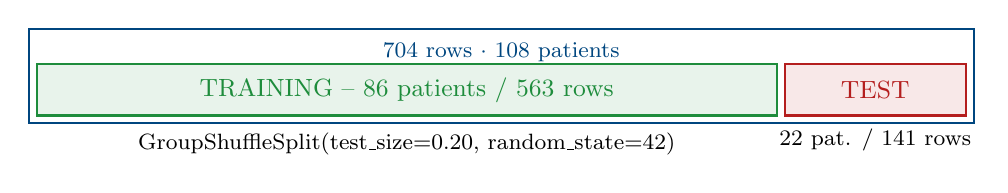
\begin{tikzpicture}[node distance=0.4cm and 0.3cm, font=\small]
  \draw[primaryblue, thick] (0,0) rectangle (12,1.2);
  \node[primaryblue] at (6,0.9) {\footnotesize 704 rows $\cdot$ 108 patients};
  \draw[successgreen, thick, fill=successgreen!10] (0.1,0.1) rectangle (9.5,0.75);
  \node[successgreen] at (4.8,0.42) {TRAINING -- 86 patients / 563 rows};
  \draw[accentred, thick, fill=accentred!10] (9.6,0.1) rectangle (11.9,0.75);
  \node[accentred] at (10.75,0.42) {TEST};
  \node[below] at (10.75,0.05) {\footnotesize 22 pat. / 141 rows};
  \node[below] at (4.8,0.0) {\footnotesize GroupShuffleSplit(test\_size=0.20, random\_state=42)};
\end{tikzpicture}
\vspace{0.5em}

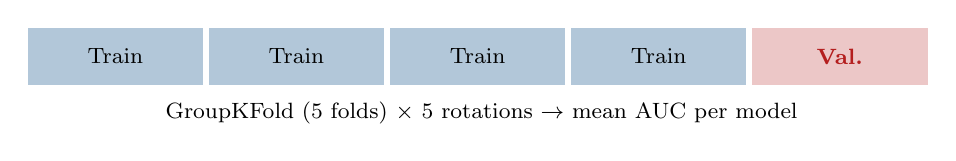
\begin{tikzpicture}[node distance=0.3cm, font=\small]
  \foreach \i/\c in {0/primaryblue!30, 1/primaryblue!30, 2/primaryblue!30, 3/primaryblue!30, 4/accentred!25} {
    \pgfmathsetmacro{\x}{\i * 2.3}
    \draw[\c, thick, fill=\c] (\x, 0) rectangle (\x+2.2, 0.7);
  }
  \node at (0*2.3+1.1, 0.35) {\footnotesize Train};
  \node at (1*2.3+1.1, 0.35) {\footnotesize Train};
  \node at (2*2.3+1.1, 0.35) {\footnotesize Train};
  \node at (3*2.3+1.1, 0.35) {\footnotesize Train};
  \node[accentred] at (4*2.3+1.1, 0.35) {\footnotesize \textbf{Val.}};
  \node[below] at (5.75, -0.1) {\footnotesize GroupKFold (5 folds) $\times$ 5 rotations $\to$ mean AUC per model};
\end{tikzpicture}
\caption{Validation strategy: patient-level 80/20 split followed by 5-fold GroupKFold cross-validation on the training set.}
\label{fig:cv}
\end{figure}

The training set (86 patients, 563 cycles) is used for all cross-validation and model selection. The test set (22 patients, 141 cycles) is completely isolated and is evaluated only once, at the end.

\section{Models}

Four ensemble classifiers were evaluated:

\begin{table}[H]
\centering
\caption{Models and hyperparameters}
\label{tab:models}
\begin{tabular}{llp{5.5cm}}
\toprule
\textbf{Model} & \textbf{Library} & \textbf{Key parameters} \\
\midrule
Random Forest & scikit-learn & 300 trees, \texttt{class\_weight=\textquotesingle{}balanced\textquotesingle{}} \\
Extra Trees & scikit-learn & 300 trees, \texttt{class\_weight=\textquotesingle{}balanced\textquotesingle{}} \\
XGBoost & xgboost & 300 iterations, \texttt{max\_depth=4}, \texttt{lr=0.05}, \texttt{scale\_pos\_weight=neg/pos} \\
LightGBM & lightgbm & 300 iterations, \texttt{max\_depth=4}, \texttt{lr=0.05}, \texttt{class\_weight=\textquotesingle{}balanced\textquotesingle{}} \\
\bottomrule
\end{tabular}
\end{table}

Within each cross-validation fold, a clone of the estimator (\texttt{sklearn.base.clone}) is trained to avoid state accumulation across folds.

\section{Ensemble Construction (Soft Voting)}

After cross-validation, the three models with the highest \emph{mean CV AUC-ROC across the five targets} are selected as ensemble members. Selection is based solely on cross-validation results---the test set is never consulted. The selected models are then retrained on the \emph{full} training set, and their predicted probabilities are averaged (soft voting):
\[
\hat{p}_{\text{ens}} = \frac{1}{3} \sum_{k=1}^{3} \hat{p}_k
\]

Averaging probabilities preserves confidence information and outperforms hard majority-vote ensembles for calibrated classifiers.

In this experiment, the top 3 models by mean CV AUC were:
\begin{center}
\textbf{XGBoost (0.9767)} $\approx$ \textbf{LightGBM (0.9756)} $\approx$ \textbf{Random Forest (0.9750)}
\end{center}
Extra Trees (mean CV AUC\,=\,0.938) was excluded from the ensemble.

\section{Evaluation Metrics}

For each target independently, the following metrics are computed on the isolated test set:
\begin{itemize}
  \item \textbf{AUC-ROC}: area under the ROC curve. Threshold-independent; suited to imbalanced classes. Primary metric.
  \item \textbf{Sensitivity (Recall)}: $\text{TP} / (\text{TP} + \text{FN})$. Proportion of true complications detected. Clinically the most important---a missed complication is more dangerous than a false alarm.
  \item \textbf{Specificity}: $\text{TN} / (\text{TN} + \text{FP})$. Proportion of non-events correctly identified as negative.
  \item \textbf{PPV (Precision)}: $\text{TP} / (\text{TP} + \text{FP})$. When the model flags a patient, how often is it right?
  \item \textbf{F1 score}: harmonic mean of sensitivity and PPV. Balanced summary for imbalanced classes.
\end{itemize}
Binary predictions are produced at a threshold of 0.50 applied to the ensemble probabilities.

\section{Feature Importance}

Post-hoc feature importance is computed using the Mean Decrease in Impurity (MDI) of the Random Forest, trained on the full training set. MDI measures how much each feature reduces impurity (Gini) across all trees, on average.

% ══════════════════════════════════════════════════════════════════════════════
\chapter{Results}
\label{chap:results}
% ══════════════════════════════════════════════════════════════════════════════

\section{Cross-Validation Results}

Table~\ref{tab:cv} reports the AUC-ROC from the 5-fold GroupKFold cross-validation on the training set (mean $\pm$ standard deviation across folds). Folds where the validation set contained only one class are excluded from the AUC computation.

\begin{table}[H]
\centering
\caption{5-fold GroupKFold cross-validation AUC-ROC (training set, mean ± SD)}
\label{tab:cv}
\setlength{\tabcolsep}{4pt}
\begin{tabular}{lccccc}
\toprule
\textbf{Model} & \textbf{Anaemia} & \textbf{Neutropenia} & \textbf{Thrombocy.} & \textbf{Renal} & \textbf{Hepatic} \\
\midrule
Random Forest & $0.969 \pm 0.012$ & $0.976 \pm 0.036$ & $0.995 \pm 0.002$ & $0.952 \pm 0.086$ & $0.983 \pm 0.015$ \\
Extra Trees   & $0.964 \pm 0.009$ & $0.909 \pm 0.090$ & $0.977 \pm 0.010$ & $0.928 \pm 0.089$ & $0.913 \pm 0.025$ \\
XGBoost       & $0.979 \pm 0.011$ & $0.993 \pm 0.012$ & $0.997 \pm 0.003$ & $0.930 \pm 0.094$ & $0.984 \pm 0.011$ \\
LightGBM      & $0.980 \pm 0.013$ & $0.996 \pm 0.008$ & $0.997 \pm 0.002$ & $0.923 \pm 0.102$ & $0.983 \pm 0.014$ \\
\midrule
\textbf{Mean} & & & & & \\
Random Forest & \multicolumn{5}{c}{0.9750 $\leftarrow$ \textbf{in the ensemble}} \\
Extra Trees   & \multicolumn{5}{c}{0.9383} \\
XGBoost       & \multicolumn{5}{c}{0.9767 $\leftarrow$ \textbf{in the ensemble}} \\
LightGBM      & \multicolumn{5}{c}{0.9756 $\leftarrow$ \textbf{in the ensemble}} \\
\bottomrule
\end{tabular}
\end{table}

The three gradient-boosting and forest models reach almost identical mean CV AUCs. Extra Trees is excluded from the ensemble because of markedly lower performance on neutropenia and thrombocytopenia.

\section{Individual Model Test-Set Performance}

\begin{table}[H]
\centering
\caption{Individual model AUC on the isolated test set (22 patients, 141 cycles)}
\label{tab:individual}
\begin{tabular}{lccccc}
\toprule
\textbf{Model} & \textbf{Anaemia} & \textbf{Neutropenia} & \textbf{Thrombocy.} & \textbf{Renal} & \textbf{Hepatic} \\
\midrule
XGBoost       & 0.998 & 0.847 & 0.991 & 0.999 & 0.976 \\
LightGBM      & 0.997 & 0.850 & 0.993 & 0.996 & 0.981 \\
Random Forest & 0.971 & 0.958 & 0.993 & 0.998 & 0.972 \\
\midrule
\textbf{Ensemble} & \textbf{0.995} & \textbf{0.954} & \textbf{0.993} & \textbf{0.999} & \textbf{0.972} \\
\bottomrule
\end{tabular}
\end{table}

The soft-voting ensemble produces AUCs comparable or superior to the best individual model on the majority of targets and offers increased robustness thanks to the averaging of calibrated probability estimates.

\section{Ensemble Test-Set Performance (Full Metrics)}

\begin{table}[H]
\centering
\rowcolors{2}{lightgray}{white}
\caption{Longitudinal ensemble performance on the isolated test set}
\label{tab:main}
\begin{tabular}{lccccccccr}
\toprule
\textbf{Complication} & \textbf{AUC} & \textbf{Sens.} & \textbf{Spec.} & \textbf{PPV} & \textbf{F1} & \textbf{TP} & \textbf{FP} & \textbf{TN} & \textbf{FN} \\
\midrule
Anaemia            & 0.995 & 1.000 & 0.887 & 0.936 & 0.967 & 88 & 6  & 47  & 0 \\
Neutropenia        & 0.954 & 0.500 & 1.000 & 1.000 & 0.667 & 2  & 0  & 137 & 2 \\
Thrombocytopenia   & 0.993 & 1.000 & 0.984 & 0.882 & 0.938 & 15 & 2  & 124 & 0 \\
Renal toxicity     & 0.999 & 0.909 & 1.000 & 1.000 & 0.952 & 10 & 0  & 130 & 1 \\
Hepatic toxicity   & 0.972 & 0.955 & 0.990 & 0.977 & 0.966 & 42 & 1  & 96  & 2 \\
\midrule
\rowcolor{primaryblue!10}
\textbf{Mean} & \textbf{0.983} & \textbf{0.873} & \textbf{0.972} & \textbf{0.959} & \textbf{0.898} & & & & \\
\bottomrule
\end{tabular}
\end{table}

\subsection{Per-Complication Interpretation}

\textbf{Anaemia} (AUC\,=\,0.995, Sensitivity\,=\,100\%): The model identifies every anaemic cycle in the test set (88/88). Six non-anaemic cycles are incorrectly flagged (false positives). Given the 68\% prevalence, this means that 6 of the 53 truly negative cycles generate false alarms---an acceptable trade-off for complete detection.

\textbf{Neutropenia} (AUC\,=\,0.954, Specificity\,=\,100\%): With only 4 positive cases in the test set (prevalence 5.1\%), this is the most difficult target. The model achieves perfect specificity (no false alarms) but misses 2 of the 4 events (sensitivity\,=\,50\%). The high AUC (0.954) indicates excellent discrimination, but the 0.50 probability threshold is conservative given the severe class imbalance.

\textbf{Thrombocytopenia} (AUC\,=\,0.993, Sensitivity\,=\,100\%): All 15 positive cases are detected, with 2 false positives. This is an excellent result for a complication with a prevalence of 17.9\%.

\textbf{Renal toxicity} (AUC\,=\,0.999, PPV\,=\,100\%): Only 1 of the 11 positive cases is missed, and there are no false alarms. The model is highly reliable for clinical use on this target.

\textbf{Hepatic toxicity} (AUC\,=\,0.972, Sensitivity\,=\,95.5\%): 42 of the 44 positive cases are detected, 2 are missed, with 1 false alarm. An excellent balance between sensitivity and specificity for the second most prevalent complication (28.6\%).

\section{Feature Importance}

\begin{figure}[H]
\centering
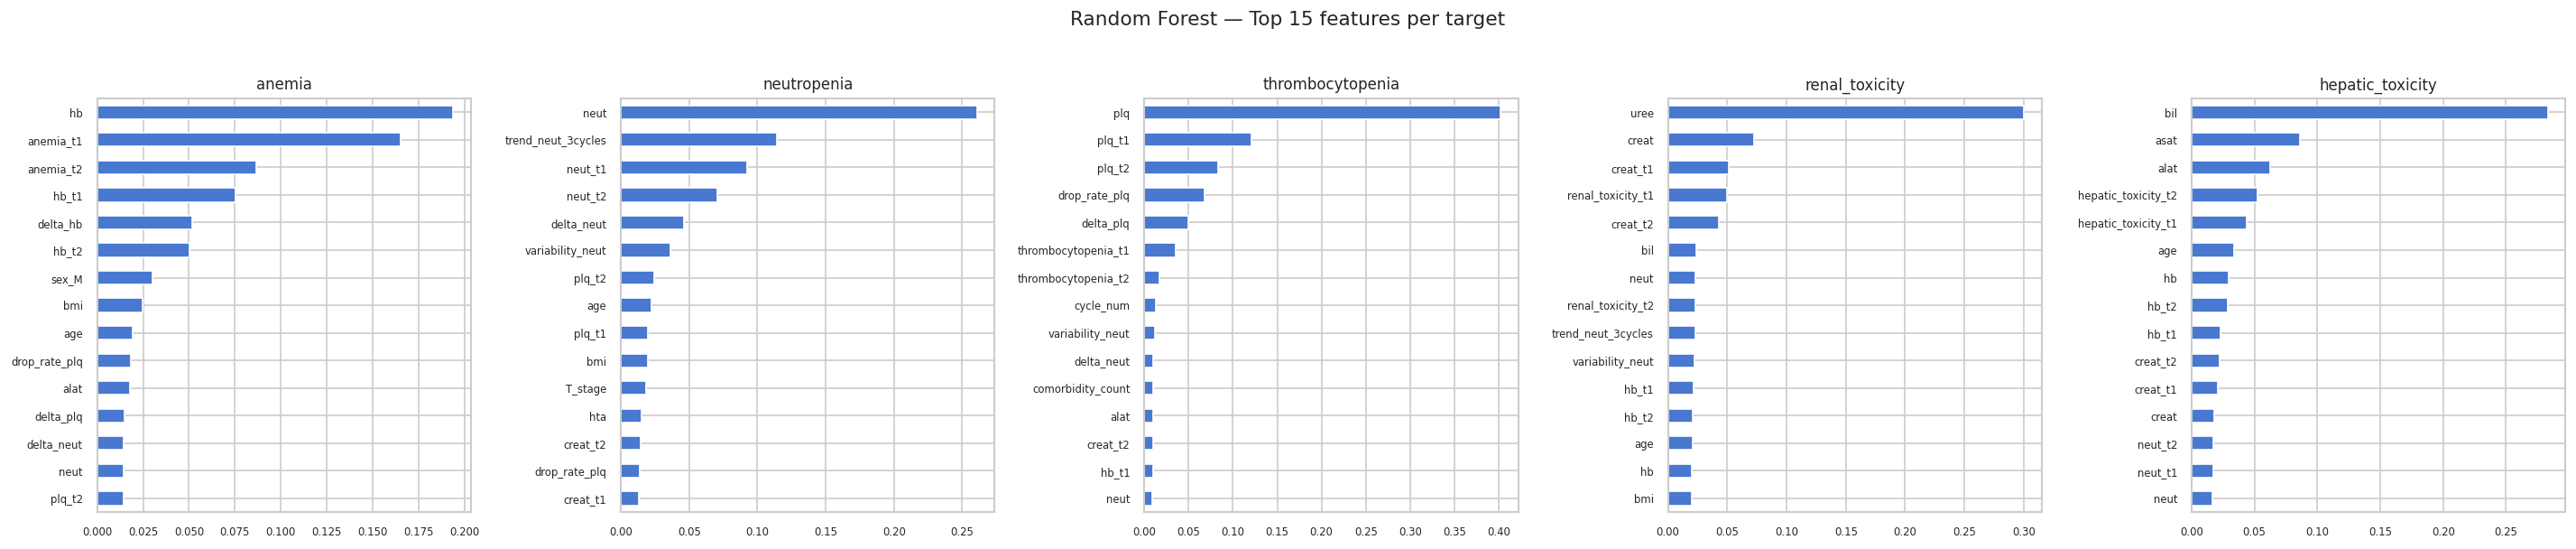
\includegraphics[width=\linewidth]{../outputs/feature_importance_longitudinal.png}
\caption{Mean Decrease in Impurity (MDI) of the Random Forest -- top 15 features per complication target, trained on the full training set.}
\label{fig:fi}
\end{figure}

The feature importance analysis in Figure~\ref{fig:fi} reveals a consistent pattern across the five targets: the \textbf{prior-complication indicators} (\texttt{anemia\_t1}, \texttt{neutropenia\_t1}, \texttt{hepatic\_toxicity\_t1}) and the \textbf{lagged biomarkers} (\texttt{hb\_t1}, \texttt{neut\_t1}, \texttt{plq\_t1}) dominate the rankings. This validates the central hypothesis of the project: what happened at the previous cycle is the best predictor of what will happen at the current cycle.

The delta features (\texttt{delta\_hb}, \texttt{delta\_neut}) appear among the top ranks for the corresponding targets, confirming that the direction and speed of change provide additional predictive value beyond the absolute lagged value.

The demographic and staging features (age, T\_stage, N\_stage) contribute less than the biological history for all targets, suggesting that within-patient temporal dynamics are more informative than static between-patient characteristics for predicting short-term complications.

\section{Per-Patient Predictions}

The file \texttt{outputs/per\_patient\_predictions.csv} contains, for each of the 141 cycles of the test set, the actual outcome and the probability predicted by the ensemble for the five complications. This table allows the clinical supervisor to verify the plausibility of the model on individual patients.

\begin{table}[H]
\centering
\caption{Example rows from the per-patient prediction table (test set)}
\label{tab:predictions}
\setlength{\tabcolsep}{3pt}
\begin{tabular}{llccccc}
\toprule
\textbf{Patient} & \textbf{Cycle} & \textbf{P(Anaemia)} & \textbf{P(Neutr.)} & \textbf{P(Thrombo.)} & \textbf{P(Renal)} & \textbf{P(Hepatic)} \\
\midrule
P1  & 2 & 0.987\,\checkmark & 0.013 & 0.012 & 0.009 & 0.045 \\
P1  & 3 & 0.989\,\checkmark & 0.017 & 0.032 & 0.015 & 0.055 \\
P1  & 4 & 0.987\,\checkmark & 0.019 & 0.874\,\checkmark & 0.015 & 0.034 \\
P108 & 2 & 0.182 & 0.008 & 0.009 & 0.005 & \textbf{0.875}\,\checkmark \\
P108 & 3 & 0.147 & 0.016 & 0.014 & 0.008 & \textbf{0.943}\,\checkmark \\
\bottomrule
\multicolumn{7}{l}{\small \checkmark = true positive (complication occurred). Bold = high probability flagged.}
\end{tabular}
\end{table}

% ══════════════════════════════════════════════════════════════════════════════
\chapter{Discussion}
\label{chap:discussion}
% ══════════════════════════════════════════════════════════════════════════════

\section{Why Do Longitudinal Features Work?}

The dominant predictors across the five complications are the prior-complication indicators and the lagged biomarkers---not the current-cycle values or the static patient characteristics. This is clinically intuitive: a patient who had anaemia at the previous cycle very probably has anaemia again; a patient whose neutrophils are steadily falling is at high risk of neutropenia.

The delta and trend features add a second layer of signal: they encode the \emph{speed} and \emph{momentum} of biological change. A current haemoglobin of 11\,g/dL is interpreted very differently depending on whether it has fallen by 2\,g/dL from the previous cycle (\texttt{delta\_hb}\,=\,-2) or has been stable at 11 for three cycles.

\section{Clinical Implications}

\subsection{For High-Prevalence Complications (Anaemia, Hepatic Toxicity)}
The model achieves near-perfect sensitivity (100\% and 95.5\% respectively) with very few false positives. These two complications account for the majority of the clinical burden (68\% and 28.6\% prevalence). The model is directly actionable for these targets: a high predicted probability should prompt the oncologist to consider haematopoietic support or liver function monitoring before the next cycle.

\subsection{For Rare Complications (Neutropenia, Renal Toxicity)}
Sensitivity for neutropenia is 50\% at the 0.50 threshold. However, when the model flags a cycle as neutropenic, it is always right (PPV\,=\,100\%). Lowering the threshold would increase sensitivity at the cost of false alarms. The AUC of 0.954 indicates that the underlying discrimination is strong, and the threshold should be tuned in a prospective setting guided by the clinical cost of a missed neutropenia versus an unnecessary G-CSF prescription.

Renal toxicity shows the best discrimination (AUC\,=\,0.999) with only 1 missed event. The model can be used with high confidence for renal monitoring.

\subsection{Proposed Clinical Workflow}

\begin{enumerate}
  \item \textbf{Cycles 1 and 2:} no prediction available (insufficient history). Standard clinical monitoring applies.
  \item \textbf{Cycle $\geq$ 3:} before the cycle is administered, enter the patient's current biomarkers and dose into the prediction system. The output is a probability for each of the five complications.
  \item \textbf{Action thresholds} (suggested, pending prospective validation):
    \begin{itemize}
      \item $\hat{p} \geq 0.50$: flag for discussion; consider a dose adjustment or prophylactic treatment.
      \item $\hat{p} \geq 0.80$: strong flag; recommend enhanced monitoring or supportive treatment.
    \end{itemize}
\end{enumerate}

\section{Limitations}

\subsection{Sample Size}
The cohort of 108 patients is small, particularly for rare events. With only 36 neutropenic cycles in the full dataset and $\approx$4 in the test set, the performance estimate for neutropenia has high variance. Confidence intervals on the test-set metrics would be very wide.

\subsection{Single-Centre Retrospective Design}
All the data come from a single hospital. The model may overfit to centre-specific practices (drug preparation, measurement instruments, threshold definitions) and may not generalise to other centres without retraining. Prospective evaluation at an independent centre is the essential next step.

\subsection{Severity Not Modelled}
The targets are binary (present/absent). FOLFOX complications range from grade I (mild, no action required) to grade IV (life-threatening, requiring hospitalisation). The current model does not distinguish severity, which limits its clinical usefulness for dose management decisions.

\subsection{Suspicious Creatinine Values}
Approximately 20 rows have creatinine values above 13\,mg/L that may represent unit errors (µmol/L entered instead of mg/L). These were retained pending clinical confirmation but may introduce noise into the renal toxicity target.

\subsection{Missing History for Cycles 1--2}
The longitudinal model cannot be applied to the first two cycles of a patient's treatment. For a 12-cycle regimen, this means that 17\% of all cycles are not covered.

\section{Future Work}

\begin{itemize}
  \item \textbf{External validation:} collect data from a second centre and evaluate the trained model without retraining.
  \item \textbf{Severity prediction:} reformulate as ordinal (grade 0--IV) or multi-class classification.
  \item \textbf{Threshold optimisation:} use Youden's J statistic to select the optimal threshold per complication based on clinical cost weighting.
  \item \textbf{Hospital information system integration:} connect the model to the laboratory information system for real-time predictions as laboratory results arrive.
  \item \textbf{Prospective trial:} randomise patients between model-guided management and standard management and measure differences in outcomes (dose reduction rate, hospitalisation rate, quality-of-life scores).
  \item \textbf{Sequence models:} with a larger dataset, LSTM or Transformer architectures could capture more complex temporal patterns than the explicit feature engineering approach.
\end{itemize}

% ══════════════════════════════════════════════════════════════════════════════
\chapter{Conclusion}
\label{chap:conclusion}
% ══════════════════════════════════════════════════════════════════════════════

This project demonstrates that a modest retrospective dataset of 108 patients on FOLFOX chemotherapy, combined with careful longitudinal feature engineering and a leakage-free ensemble methodology, is sufficient to build a clinically convincing predictive system for biological complications.

The central finding is that \textbf{the history of prior complications and the lagged biomarkers are the dominant predictors}---not the static demographic data nor the current laboratory results alone. This validates the longitudinal approach and motivates the explicit encoding of the patient's trajectory as concrete numerical features.

The resulting ensemble (XGBoost + LightGBM + Random Forest, soft voting) achieves a \textbf{mean AUC-ROC of 0.983} across five complications on 22 unseen patients. For the clinically critical complications, the model reaches perfect or near-perfect sensitivity: anaemia (100\%), thrombocytopenia (100\%), hepatic toxicity (95.5\%) and renal toxicity (90.9\%). Neutropenia, the rarest and most dangerous event, reaches an AUC\,=\,0.954 with a perfect PPV---every alarm raised for neutropenia corresponds to a real event.

All the code, (anonymised) data, trained models and documentation are provided in the project deliverables, making the system fully reproducible and ready for prospective validation.

% ══════════════════════════════════════════════════════════════════════════════
%  REFERENCES
% ══════════════════════════════════════════════════════════════════════════════
\chapter*{References}
\addcontentsline{toc}{chapter}{References}

\begin{enumerate}[label={[\arabic*]}]
  \item André T, Boni C, Mounedji-Boudiaf L, et al. Oxaliplatin, fluorouracil, and leucovorin as adjuvant treatment for colon cancer. \textit{N Engl J Med.} 2004;350(23):2343--2351.
  \item Cassidy J, Clarke S, Díaz-Rubio E, et al. Randomized phase III study of capecitabine plus oxaliplatin compared with fluorouracil/folinic acid plus oxaliplatin as first-line therapy for metastatic colorectal cancer. \textit{J Clin Oncol.} 2008;26(12):2006--2012.
  \item Common Terminology Criteria for Adverse Events (CTCAE) v5.0. National Cancer Institute, 2017.
  \item Breiman L. Random forests. \textit{Mach Learn.} 2001;45(1):5--32.
  \item Chen T, Guestrin C. XGBoost: A scalable tree boosting system. \textit{KDD 2016.} 785--794.
  \item Ke G, Meng Q, Finley T, et al. LightGBM: A highly efficient gradient boosting decision tree. \textit{NeurIPS 2017.}
  \item Pedregosa F, et al. Scikit-learn: Machine learning in Python. \textit{JMLR.} 2011;12:2825--2830.
  \item Strobl C, Boulesteix AL, Zeileis A, Hothorn T. Bias in random forest variable importance measures. \textit{BMC Bioinformatics.} 2007;8:25.
\end{enumerate}

% ══════════════════════════════════════════════════════════════════════════════
%  APPENDICES
% ══════════════════════════════════════════════════════════════════════════════
\appendix

\chapter{Data Dictionary}
\label{app:dict}

The complete data dictionary for \texttt{dataset\_longitudinal.csv} (704 rows $\times$ 59 columns) is reproduced below in summary form. For the full version, see \texttt{data/data\_dictionary.md}.

\begin{longtable}{p{3.5cm}p{1.5cm}p{2.5cm}p{5.5cm}}
\caption{Data dictionary summary} \label{tab:dict} \\
\toprule
\textbf{Column} & \textbf{Type} & \textbf{Unit / Values} & \textbf{Description} \\
\midrule
\endfirsthead
\toprule \textbf{Column} & \textbf{Type} & \textbf{Unit / Values} & \textbf{Description} \\ \midrule
\endhead
\midrule \multicolumn{4}{r}{\small Continued on next page} \\
\endfoot
\bottomrule
\endlastfoot
patient\_id & string & P1\ldots P109 & Patient identifier (not used as a feature) \\
cycle\_num & integer & 0--17 & Cycle number ($\geq$2 in this dataset) \\
age & integer & years & Age at first cycle \\
sex\_M & binary & 0/1 & 1 = male \\
bmi & float & kg/m² & Body mass index \\
etat & category & 0/1/2 & Nutritional status (ordinal) \\
hta & binary & 0/1 & Arterial hypertension \\
diabetes & binary & 0/1 & Diabetes \\
renal\_disease & binary & 0/1 & Chronic kidney disease \\
hepatic\_disease & binary & 0/1 & Chronic liver disease \\
comorbidity\_count & integer & 0--4 & Sum of the four comorbidities \\
cancer\_type & category & Colon/\ldots & Tumour location \\
T\_stage & integer & 0--4 & T stage (TNM) \\
N\_stage & integer & 0--4 & N stage (TNM) \\
M\_stage & integer & 0--1 & M stage (TNM) \\
has\_metastasis & binary & 0/1 & Metastatic disease \\
treatment\_intent & category & Adj/Neoadj & Treatment intent \\
interval\_days & integer & days & Days since the previous cycle \\
dose\_oxali & float & mg/m² & Oxaliplatin dose \\
dose\_5fu\_bolus & float & mg/m² & 5-FU bolus dose \\
dose\_5fu\_cont & float & mg/m² & Continuous 5-FU infusion dose \\
dose\_af & float & mg/m² & Folinic acid dose \\
hb & float & g/dL & Haemoglobin (current) \\
neut & float & G/L & Neutrophils (current) \\
plq & float & G/L & Platelets (current) \\
uree & float & g/L & Urea \\
creat & float & mg/L & Creatinine \\
asat & float & IU/L & AST \\
alat & float & IU/L & ALT \\
bil & float & mg/L & Total bilirubin \\
hb\_t1/t2 & float & g/dL & Hb one/two cycles earlier \\
neut\_t1/t2 & float & G/L & Neutrophils one/two cycles earlier \\
plq\_t1/t2 & float & G/L & Platelets one/two cycles earlier \\
creat\_t1/t2 & float & mg/L & Creatinine one/two cycles earlier \\
anemia\_t1/t2 & binary & 0/1 & Anaemia occurred at t-1/t-2 \\
neutropenia\_t1/t2 & binary & 0/1 & Neutropenia at t-1/t-2 \\
thrombocyt.\_t1/t2 & binary & 0/1 & Thrombocytopenia at t-1/t-2 \\
renal\_tox.\_t1/t2 & binary & 0/1 & Renal toxicity at t-1/t-2 \\
hepatic\_tox.\_t1/t2 & binary & 0/1 & Hepatic toxicity at t-1/t-2 \\
delta\_hb & float & g/dL & $\texttt{hb} - \texttt{hb\_t1}$ \\
delta\_neut & float & G/L & $\texttt{neut} - \texttt{neut\_t1}$ \\
delta\_plq & float & G/L & $\texttt{plq} - \texttt{plq\_t1}$ \\
trend\_neut\_3cycles & float & G/L & 3-cycle mean of neutrophils \\
drop\_rate\_plq & float & ratio & $(plq - plq_{t2}) / plq_{t2}$ \\
variability\_neut & float & G/L & 3-cycle standard deviation of neutrophils \\
target\_anemia & binary & 0/1 & \textbf{Target}: anaemia this cycle \\
target\_neutropenia & binary & 0/1 & \textbf{Target}: neutropenia this cycle \\
target\_thrombocyt. & binary & 0/1 & \textbf{Target}: thrombocytopenia \\
target\_renal\_tox. & binary & 0/1 & \textbf{Target}: renal toxicity \\
target\_hepatic\_tox. & binary & 0/1 & \textbf{Target}: hepatic toxicity \\
\end{longtable}

\chapter{Reproducibility}
\label{app:repro}

\section{Software Environment}

\begin{lstlisting}
Python         3.12
pandas         >= 2.0
numpy          >= 1.24
scikit-learn   >= 1.3
xgboost        >= 2.0
lightgbm       >= 4.0
joblib         >= 1.3
matplotlib     >= 3.7
seaborn        >= 0.12
jupyter        >= 1.0
nbconvert      >= 7.0
\end{lstlisting}

\section{Running the Pipeline}

\begin{lstlisting}[language=bash]
# Install dependencies
pip install -r requirements.txt

# Step 1: Build the longitudinal dataset
jupyter nbconvert --to notebook --execute --inplace \
  notebooks/1_data_preparation.ipynb

# Step 2: Model training and evaluation
jupyter nbconvert --to notebook --execute --inplace \
  notebooks/2_model_longitudinal.ipynb
\end{lstlisting}

The two notebooks are fully self-contained and will reproduce all the tables and figures in this report.

\chapter{Project File Structure}
\label{app:files}

\begin{lstlisting}
oncolab-ai/
|-- data/
|   |-- raw/
|   |   `-- Collect Data Onco Lab AI - Feuille 2.csv
|   |-- dataset_longitudinal.csv      (704 x 59)
|   `-- data_dictionary.md
|-- notebooks/
|   |-- 1_data_preparation.ipynb
|   `-- 2_model_longitudinal.ipynb
|-- models/
|   |-- anemia_LightGBM.pkl
|   |-- anemia_XGBoost.pkl
|   |-- anemia_RandomForest.pkl
|   |   ... (15 files: 3 models x 5 targets)
|-- outputs/
|   |-- feature_importance_longitudinal.png
|   `-- per_patient_predictions.csv
|-- report/
|   |-- report_fr.tex
|   `-- thesis.md
|-- README.md
`-- requirements.txt
\end{lstlisting}

\end{document}
